\documentclass[11pt,reqno]{amsart}
\usepackage[top=1in, left=1in, right=1in, bottom=1in]{geometry}                % See geometry.pdf to learn the layout options. There are lots.
\geometry{letterpaper}                   % ... or a4paper or a5paper or ...
\usepackage[parfill]{parskip}    % Activate to begin paragraphs with an empty line rather than an indent

\usepackage{algorithm}
\usepackage{algpseudocode}
\usepackage{hyperref}
\usepackage{graphicx}
\usepackage{url}
\usepackage{verbatim}
\usepackage{amssymb}
\usepackage{amsaddr}
\usepackage{amsmath}
\usepackage{enumitem}
\usepackage{setspace}
\usepackage{natbib}


\newcommand{\RR}{I\!\!R} %real numbers
\DeclareMathOperator{\diag}{diag}

\algnewcommand{\Inputs}[1]{%
  \State \textbf{Inputs:}
  \Statex \hspace*{\algorithmicindent}\parbox[t]{.8\linewidth}{\raggedright #1}
}
\algnewcommand{\Initialize}[1]{%
  \State \textbf{Initialize:}
  \Statex \hspace*{\algorithmicindent}\parbox[t]{.8\linewidth}{\raggedright #1}
}


\title[Reveiw on RVD Methods]{Review on rare variant detection methods for next-generation sequencing data}
\author[F. Zhang AND P. Flaherty]{Fan Zhang\,$^{1}$, Patrick Flaherty\,$^{1,2}$}
\address{$^{1}$Department of Biomedical Engineering, Worcester Polytechnic Institute, MA, USA\\
$^{2}$Department of Mathematics and Statistics, University of Massachusetts, Amherst, MA, USA}

\begin{document}
\maketitle

\section{Introduction}
%\subsection{Sequence Analysis Pipeline}
%Review http://www.ncbi.nlm.nih.gov/pmc/articles/PMC4179624/

%Scope the article to nucleotides and variant calling in the context of larger pipeline.
Next-generation sequencing (NGS) technology has revealed the presence of extensive genomic variants in clinical samples.
The general pipeline to analyze single nucleotide variants (SNVs) in the large-scale NGS data basically consists five main steps: quality control, preprocessing, alignment, post-alignment processing, and variant detection \citep{Bao2014}.
In this sequence analysis pipeline, variant detection is the last and the most important step for discovering disease-causing variants.
In this review, we focus on rare variant detection in the DNA sequencing data and classification of current computational and statistical variant detection methods.

%Outline the paper here with one paragraph overview per section.
We first highlight the necessity of a sensitive variant detection method from the perspective of biological impacts and statistical accuracy,
and then present the hallmarks of a good variant detection method based on the evaluation of accuracy, scalability, and robustness.
We also discuss the issues that will effect the ability of variant detection methods.
Finally, we classify the state-of-the-art variant detection methods into the categories of probabilistic or non-probabilistic methods and survey each method in detail.


\section{Why do we need a sensitive variant detection method?}

Motivation

Biological impacts.

Statistical accuracy.

What is the payoff for spending time and energy on this problem.



%\subsection{Variants}
%\subsubsection{Germline, somatic, or LOH (loss of heterozygosity)}
%\subsubsection{Rare and common variants}

\section{Hallmarks of a good variant detection method}
\subsection{Accuracy}
\subsection{Scalability}
\subsection{Robustness}

It depends on specific purposes.

\section{Factors that effect the ability of variant detection methods}
coverage of NGS data, allele fraction...



\section{Classification for variant detection methods}
We classify the state-of-the-art variant detection methods into two categories - probabilistic methods and non-probabilistic methods (Table~\ref{tbl:methods}).
\begin{table}[htbp]
\centering
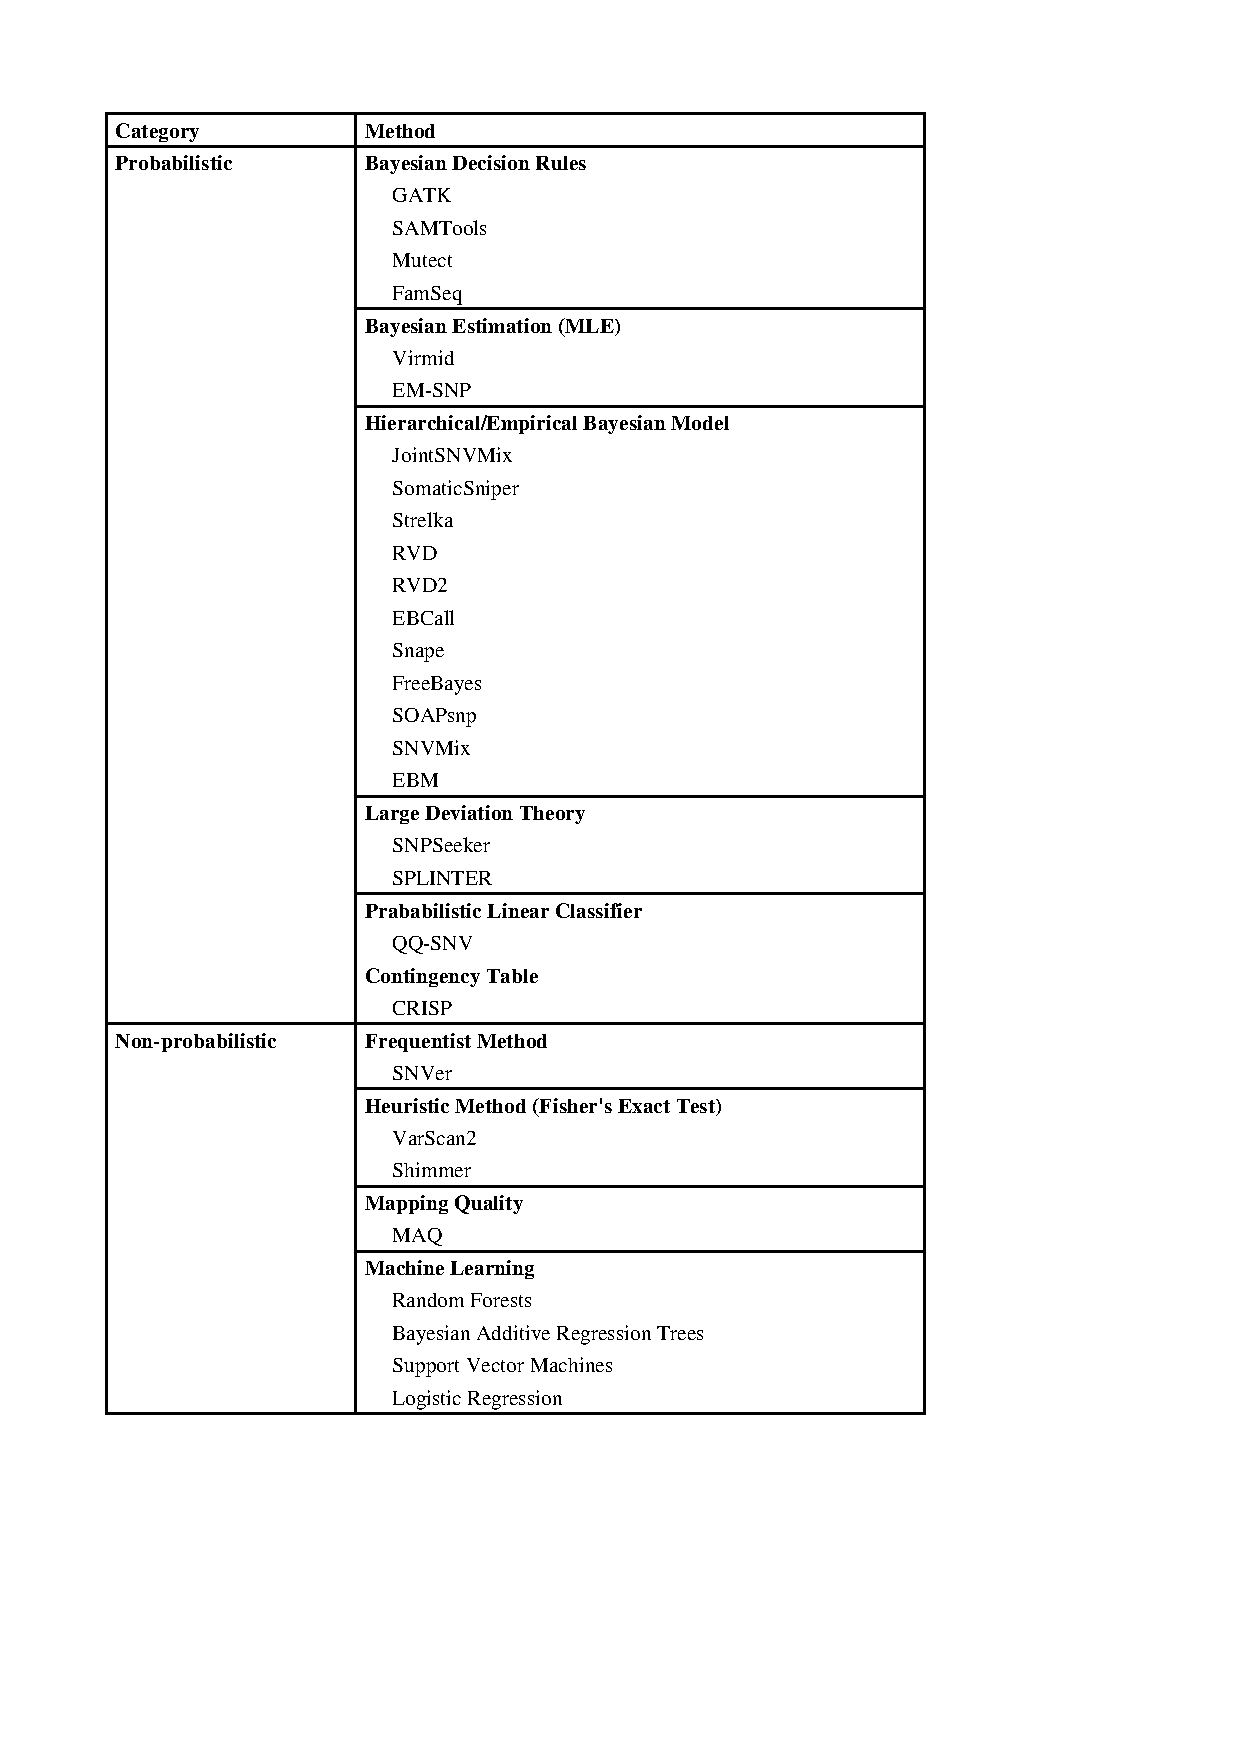
\includegraphics[width=1.2\textwidth]{method_table.pdf}
\caption{Single nucleotide variant detection methods.}
\label{tbl:methods}
\end{table}


\subsection{Probabilistic Methods}
List of 21 probabilistic methods for variant detection:

- one sentence purpose of the methods

- categories that the method falls into

- metrics and application

GATK \citep{McKenna2010},



SAMTools \citep{Li2009a},

Mutect \citep{Cibulskis2013},

FamSeq \citep{Peng2013},

Virmid \citep{Kim2013},

EM-SNP \citep{Chen2013},

JointSNVMix \citep{Roth2012},

SomaticSniper \citep{Larson2012},

Strelka \citep{Saunders2012},

RVD \citep{Flaherty2012},

RVD2 \citep{He2015},

EBCall \citep{Shiraishi2013},

Snape \citep{Raineri2012},

FreeBayes \citep{Garrison2012},

SOAPsnp \citep{Li2009},

SNVMix \citep{Goya2010},

EBM \citep{Zhou2012},

SNPSeeker \citep{Druley2009},

SPLINTER \citep{Spencer2014},

QQ-SNV \citep{VanderBorght2015},

CRISP \citep{Bansal2010}.

\subsection{Non-probabilistic Methods}
List of 8 non-probabilistic methods for variant detection:

SNVer \citep{Wei2011},

VarScan2 \citep{Koboldt2012},

Shimmer \citep{Hansen2013},

MAQ \citep{Li2008},

Random Forests \citep{Ding2012},

Bayesian Additive Regression Trees \citep{Ding2012},

Support Vector Machines \citep{Ding2012},

Logistic Regression \citep{Ding2012}.


\bibliographystyle{apalike}
\bibliography{bib}
\end{document}
